\documentclass[11pt]{article}

\usepackage{amsmath}
\usepackage{amssymb}
\usepackage{amsfonts}
\usepackage{mathtools}

\usepackage[thmmarks, amsmath]{ntheorem}

\usepackage{graphicx}
\usepackage[a4paper]{geometry}

\usepackage{diffcoeff}
\diffdef{}{op-symbol=\mathrm{d},op-order-sep=0mu}

\usepackage{cancel}

\usepackage{enumitem}

\setlist[enumerate,1]{label=\alph*)}

\usepackage{tikz-cd}
\usetikzlibrary{positioning}
\usepackage{float}

\usepackage{fontspec}
\setmonofont{Consolas}
\usepackage{listings}
\lstset{
basicstyle=\ttfamily\footnotesize,
keepspaces=true,
tabsize=4,
breaklines=true,
moredelim=**[is][\color{blue}]{@}{@},
columns=fullflexible
}

\usepackage{hyperref}
\usepackage{xurl}

\title{Applied Category Theory\\
Monads and Haskell}
\author{Duarte Maia}
%\date{}

\theorembodyfont{\upshape}
\theoremseparator{.}
\newtheorem{theorem}{Theorem}
\newtheorem{prop}{Proposition}
\renewtheorem*{prop*}{Proposition}
\newtheorem{lemma}{Lemma}
\newtheorem{definition}{Definition}
\newtheorem{remark}{Remark}

\newtheorem{joke}{Joke}


\theoremstyle{nonumberplain}

\theoremheaderfont{\itshape}
\theorembodyfont{\upshape}
\theoremseparator{:}
\theoremsymbol{\ensuremath{\blacksquare}}
\newtheorem{proof}{Proof}

\newcommand{\R}{\mathbb{R}}
\newcommand{\C}{\mathbb{C}}

\newcommand{\PP}{\mathbb{P}}
\newcommand{\FF}{\mathcal{F}}

\newcommand{\I}{\mathrm{i}}
\newcommand{\e}{\mathrm{e}}



\DeclareMathOperator{\inte}{int}
\DeclareMathOperator{\codim}{codim}
\newcommand{\grad}{\nabla}

\DeclarePairedDelimiter{\norm}{\lvert}{\rvert}
\DeclarePairedDelimiter{\Norm}{\lVert}{\rVert}


\newcommand{\Hask}{\mathrm{Hask}}
\newcommand{\type}[1]{\mathrm{#1}}
\newcommand{\typecons}[1]{\mathop{\mathrm{#1}}}
\newcommand{\cat}[1]{\mathrm{#1}}

\newcommand{\blank}{{-}}
\newcommand{\op}{\mathrm{op}}
\newcommand{\id}{\mathrm{id}}
\newcommand{\nto}{\Rightarrow}

\DeclareMathOperator{\Hom}{Hom}

\newcommand*\lsin{\lstinline}
\newcommand*\lsmath[1]{\text{\lstinline|#1|}}


\begin{document}
\maketitle
\pagebreak

\tableofcontents
\pagebreak

\section{Introduction}

In the 1930s, around the same time as Alan Turing published his work on what we nowadays call Turing machines, Alonzo Church published his own formalism for computability, which is called \emph{lambda calculus}. Around this time, it was also proven that these two notions of computability are equivalent. Today, Turing Machines serve as the `public face' of computability: we say that a function is computable if there exists a Turing machine which computes it, for example. As far as computational models go, Turing machines are very slow and unwieldy, but they match cleanly to our mental model of what computation is: a sequence of instructions which can be followed to turn inputs into outputs.

Lambda calculus does not match our intuition as cleanly, being based on substitution of expressions in other expressions, but surprisingly turns out to be much more well behaved in practical terms. Starting with ALGOL around 1960, some programming languages have included some features originating from lambda calculus, such as first-class and anonymous functions, which will be explained later. This is especially noticeable in the programming language Haskell, whose first version was published in 1989, which at its core is simply a lambda calculus evaluator.

Lambda calculus comes in several shapes, but the kind relevant for Haskell is the so-called \emph{typed lambda calculus}. It is typed in the sense that functions have well-defined domains and codomains, which are known at compilation time, and it is a syntatic error to compose functions whose domains and codomains do not match. In other words, Haskell is \emph{strongly typed}, in opposition to C, in which a function which recieves a floating-point number may instead accept an integer. As a consequence, functions in Haskell can be thought of as forming a category, with the domain and codomain of every function being known at compile time and composition only being allowed between functions of compatible types. This is part of the reason why there is such a strong relation between Haskell and category theory.

Besides being strongly typed, another important feature of Haskell is \emph{purity}. Essentially, functions in Haskell are like mathematical functions, in the sense that the same function called with the same input will always return the same output, depending on nothing other than its input and doing nothing other than returning its output. This has wide and far-reaching consequences, both in terms of performance (since there is no implicit input or output, the compiler is free to rearrange the order of computations, or even have them done in parallel) and in terms of code maintainability (when changing pre-existing code, the developer does not need to have knowledge of any other part of the system, making it easier for several developers to work in isolation), but also means that a wide array of tools programmers rely on are inviabilized. For example, simulations of physical objects are often done by defining global variables representing the $x$ and $y$ coordinates of the objects at play, their velocities, etc., and then defining a function which advances the global state in time, calling that function on repeat until the desired amount of time has elapsed:
\begin{lstlisting}
x = 0
y = 0
vx = 0
vy = 0
t = 0
while t < 1000:
	vx, vy = force(x,y)
	x = x + vx
	y = y + vy
print("At t = 1000, the object is at " + (x,y))
\end{lstlisting}

This is impossible in Haskell, as not only can global variables never be changed, but even if they could, this could not be done inside of a function, because functions cannot modify anything, only return an output. This requires that the programmer change their perspective: in this case, instead of defining a function which \emph{modifies} a few global variables, one instead defines a function which receives as input the state of the physical system at time $t$ and returns the state at time $t + \dl t$. 

This is just an example of how purity requires a complete rearrangement of the way one thinks about a problem. In this case a solution was quickly found, but how does one receive input from the user? How does one write to a file? How does one implement an algorithm which relies on mutable state, e.g. marking the nodes of a graph as they are traversed? And most importantly, how does one do all of the above without making the code completely unreadable? This is a place where category theory has found surprising application, by providing powerful abstractions which pick up the slack left by the lack of global state and mutability, and at the same time giving Haskell unprecedented amounts of type safety and generality. In the same way that many seemingly unrelated phenomena were found by category theorists to be expressions of a single phenomenon (for example, adjunctions, limits or colimits), computer theorists have found abstractions which encompass many programming strategies which on the surface seem to be completely distinct.

In this essay, I hope to convince the reader that there are very real mathematical concepts underlying many tools used by in the day-to-day of a Haskell programmer. Furthermore, I also want to get across that these concepts are \emph{useful}, allowing for cleaner and more understandable code, at least so long as the programmer is familiar with the underlying math!

\section{A Crash Course in Haskell}

The following examples are all valid Haskell code, which was implemented and executed in GHCi, the Glasgow Haskell Compiler interpreter, which is the \textit{de facto} implementation of Haskell and can be downloaded here: \url{https://www.haskell.org/downloads/}. The reader can also try Haskell online without downloading anything on \url{https://tryhaskell.org/}.

(A disclaimer: If the reader tries the examples below, some of them might yield output which is different from the one shown, in particular in regards to types of functions. This is because some functions are much more general than we present them as, but an explanation of this generality must wait until we discuss typeclasses in \ref{sec:functors}. In any case, the reader is assured that where the output of code in this essay is wrong, it is at most a particular case of the truth.)

As mentioned in the introduction, Haskell is at its core a lambda calculus evaluator, so we begin by introducing the most basic concept to lambda calculus: the lambda expression.

\subsection{Lambda expressions}

A lambda expression is something similar to the notation $a \mapsto f(a)$ for defining mathematical functions without giving them a name. For example, if I am talking about the function which squares a given number, I may write it as $a \mapsto a^2$. A lambda expression is the same, but it is written using a slightly different notation: the square function would be written as $\lambda a. a^2$. The $\lambda$ marks the beginning of the function, then the argument is given a name, and then an expression is written, in which the only free variable is the one in the argument.

A lambda expression can be applied as a function. For example, we could write $(\lambda a. a^2) 2$; in lambda calculus, function application is written without parentheses. Whenever a lambda expression is juxtaposed to the left of another expression, it should be understood as applying the function defined by the lambda to the argument given by the expression. The above example can be written in Haskell as
\begin{lstlisting}
(\a -> a^2) 2
output: 4
\end{lstlisting}

Note the changes in syntax: the lambda has been replaced by a backslash (it's like a lambda with one leg cut off), and the period has been replaced by an arrow. Also, note that the expression \lstinline|(\a -> a^2)| represents a Haskell function, but it has not been given a name. For this reason, lambda expressions in Haskell are also called \emph{anonymous functions}.

The way that this works under the hood is that the Haskell interpreter is doing something called $\beta$-reduction. Formally, given an expression $f x$ where $f$ is a lambda expression of the form $(\lambda a. M)$, the Haskell interpreter rewrites it as $M[a=x]$, i.e. the expression $M$ where every instance of the variable $a$ has been replaced by $x$. In the above example, \lstinline|(\a -> a^2) 2| is $\beta$-reduced to \lstinline|2^2|, which is then evaluated to 4.

The reason why this idea is so powerful is the following: \emph{in Haskell and in lambda calculus, lambda expressions are first class objects}. What this means is that functions can be stored in variables and given as arguments to other functions. For example, the following lambda expression takes as an argument another lambda expression, and returns its `square'. Mathematically, we would usually write it as $f \mapsto f \circ f$.
\begin{lstlisting}
\f -> (\x -> f (f x))
\end{lstlisting}

\subsection{Variables, Syntactic Sugar and Recursion}

As we have seen, functions in Haskell do not need to be named, but that does not mean that they should not. If we want to use a function more than once, we do not want to rewrite its definition every time we do. Therefore, Haskell lets us name expressions so that we may reuse them later. For example,
\begin{lstlisting}
f = \a -> a^2
x = 2
f x
output: 4
\end{lstlisting}

It is inconvenient to write lambda expressions whenever we want to define a function, so Haskell allows us to define functions using more convenient and slightly more standard notation
\begin{lstlisting}
f a = a^2
\end{lstlisting}
though it should be understood that beneath this expression is a definition via a lambda expression. Haskell contains many of these alternative notations, in which a common but cumbersome expression is given an alternative notation, which is unfurled to its underlying meaning before being passed to the Haskell interpreter. These kind of syntactic expansion rules are collectively referred to as \emph{syntactic sugar}.

Another piece of syntactic sugar without which writing any program would be almost impossible is recursion. As an example, consider the following implementation of the factorial function
\begin{lstlisting}
factorial x = if x == 0 then 1 else x * factorial (x-1)
\end{lstlisting}

This is a valid definition in Haskell, but it is not easy to write it as a lambda expression, because the function is being called inside itself. If we were to naïvely write \lstinline|factorial| as an anonymous lambda expression, we would get
\begin{lstlisting}
\x -> if x == 0 then 1 else x * factorial (x-1),
\end{lstlisting}
which would require us to expand the definition of factorial inside the expression (since it is anonymous we cannot refer to it by name), obtaining a more complex expression which itself has a factorial, and so on. This tricky problem (expressing recursion in lambda calculus) has a solution via the so-called $Y$ combinator, which is a particular lambda expression which can be used to define the factorial as above. Fortunately, as a Haskell programmer we don't need to know about it, because recursive expressions are rewritten using the $Y$ combinator under the hood.

\subsection{Types and Morphisms}

As we said in the introduction, Haskell is strongly typed: every function has a domain and a codomain. This makes Haskell a category\footnote{This is not exactly true; see \cite{haskisnotcat}.}, which is usually called $\Hask$, in which the types (examples: \lstinline|Int|, \lstinline|Char|, \lstinline|String|) are the objects and the functions (lambda expressions) are the morphisms.

That said, what is the domain and codomain of the lambda expression \lstinline|\a -> a^2|? We have evaluated it on the number 2, which is an integer (i.e. of type \lstinline|Int|) and gotten an integer back, but we could also have applied it to the floating-point number 2.1 (of type \lstinline|Float|). We'll get back to this ambiguity later, but to assuage our concerns we can add type annotations explicitly using the following syntax
\begin{lstlisting}
f :: Int -> Int
f a = a^2
\end{lstlisting}

This means that $f$ is a morphism with domain \lstinline|Int| and codomain \lstinline|Int|; mathematically, $f \in \Hask(\type{Int}, \type{Int})$. If we try to evaluate it on a non-integer such as 2.1, we get an error:\footnote{Strictly speaking, this isn't the error you'll actually get. You'll get something like \lstinline|No instance for (Fractional Int) arising from the literal '2.1'|, which is Haskell trying a little harder to make 2.1 into an integer.}
\begin{lstlisting}
f 2.1
<interactive>:1:3: error:
    • Couldn't match expected type 'Int' with actual type 'Float'
    • In the first argument of 'f', namely '2.1'
      In the expression: f 2.1
      In an equation for 'it': it = f 2.1
\end{lstlisting}

Haskell has a wide array of so-called primitive types, like \lstinline|Int|, \lstinline|Char| and so on, but it also allows us to make complex types out of simpler ones. We have already seen one: the humble arrow!

The sequence of characters \lstinline|->| has the role usually taken by $\Hom$ or $C$ in categorical texts: we write \lsin|a -> b| to denote what we would usually call $\Hask(a,b)$. This is in itself a Haskell type. In other words, \emph{the $\Hask$ category has exponential objects}. This is the first taste of categorical language in Haskell.

\subsection{Currying and Composition}

So far, every function we have seen takes only one argument. This is also the case in lambda calculus: every lambda has exactly one variable. It also happens in, for example, the category of $\cat{Sets}$: an arrow $A \to B$ takes as argument exactly one element of $A$. Of course, we emulate our functions taking multiple arguments by using cartesian products: a function $f$ which receives two real numbers and returns another is denoted as
\begin{equation}
f \colon \R \times \R \to \R.
\end{equation}

A similar process can be done in Haskell, so that a function that receives, say, two integers, could have type \lsin|(Int,Int) -> Int|. The comma \lsin|(,)| denotes the categorical product in $\Hask$, and is another example of a type constructor. However, functions receiving multiple arguments are usually handled another way.

The type of a pre-existing function \lsin|f| can be found by writing \lsin|:t f| in GHCi. For example, using \lsin|f = (+)|, i.e. the predefined function which adds two numbers, we get\footnote{Again, the actual output isn't exactly the one shown, as addition is defined more generally than on the integers.}
\begin{lstlisting}
:t (+)
output: (+) :: Int -> Int -> Int
\end{lstlisting}

What gives? This expression will be made clearer if we introduce parentheses. Haskell associates the \lsin|->| operator to the right, so the above expression should be read as
\begin{lstlisting}
(+) :: Int -> (Int -> Int)
\end{lstlisting}

Aha! So what's happening here, in categorical terms, is simply that
\begin{equation}
(+) \in \Hask(\type{Int}, \Hask(\type{Int}, \type{Int})).
\end{equation}

Recall that, in sets, we have an adjunction between the functors
\begin{equation}
F(a) = a \times b, \quad G(c) = \Hom(b,c).
\end{equation}

In particular, $F \dashv G$, and the natural isomorphism given by the adjunction is defined as, say,
\begin{equation}
\begin{aligned}
\phi \colon \Hom(a \times b, c) &\to \Hom(a, \Hom(b,c))\\
f &\mapsto (x \mapsto (y \mapsto f(x,y))).
\end{aligned}
\end{equation}

In Haskell, this isomorphism is called \lsin|curry|. We say functions in Haskell are \emph{curried}. The nomenclature is in honor of Haskell Curry, an important logician. We can inspect the type of this function in GHCi:
\begin{lstlisting}
:t curry
output: curry :: ((a, b) -> c) -> a -> b -> c
\end{lstlisting}

This matches our expectation, but remember that parentheses are implicit on the right-hand side. Note the use of the so-called \emph{type variables}: any `type' whose name is a lower-case letter denotes a type variable, and may be substituted by any type. Therefore, \lsin|curry| isn't a function in and of itself: it is a family of functions, parametrized by three objects in $\Hask$: $a$, $b$ and $c$. This is similar to how the usual isomorphism in adjunctions is parametrized by a pair of objects, as in $\varphi_{xy}$. In Haskell, the parametrization is implicit: the compiler keeps the definition as ambiguous as possible at every moment, and deduces what $a$, $b$ and $c$ should be from context when necessary.

Surprisingly, currying (and its inverse, \lsin|uncurry|) isn't used very often. Functions are almost always left curried, because this allows for a technique called partial application. We won't go into details, but for example expressions such as \lsin|(\a -> f 2 a)| are usually shortened to \lsin|(f 2)|.

Finally, let's talk about the most important categorical concept: function composition. It is a very surprising fact that almost no modern languages have a composition operator, but Haskell does. It is denoted with a single dot, as in \lsin|f . g|, as it is the closest a standard keyboard gets to the usual notation of composition, except perhaps for the hideous notation \lsin|f o g|. Unsurprisingly, the composition has type given by
\begin{lstlisting}
:t (.)
output: (.) :: (b -> c) -> (a -> b) -> a -> c
\end{lstlisting}

Again, note the usage of type variables: the types written in lower case are a stand in for any type in $\Hask$.


\section{Elementary Categorical Concepts}

\subsection{A Few Limits and Colimits}\label{limcolim}

We have already seen a few examples of categorical concepts cropping up in Haskell. The types and morphisms form a category called $\Hask$ (kind of, see \cite{haskisnotcat}), the arrow operator \lsin|->| is the categorical exponent, the comma operator \lsin|(,)| is the categorical product, and these two functors (though we haven't realized them as functors yet) are adjoint to each other, with the bijection between hom-sets being given by \lsin|curry|.

Another common categorical construction is the coproduct. In Haskell, this is realized by using the \lsin|Either| type constructor. The coproduct of two types $a$ and $b$ is denoted \lsin|Either a b|, and the coproduct diagram is the following, with the inclusions being denoted by \lsin|Left| and \lsin|Right|.
\begin{equation}
\begin{tikzcd}[column sep = large]
\lsmath{a} \arrow[r, "\lsmath{Left}"] & \lsmath{Either a b} & \lsmath{b} \arrow[l, "\lsmath{Right}"']
\end{tikzcd}
\end{equation}

We also present the product diagram of \lsin|(a,b)|.
\begin{equation}
\begin{tikzcd}[column sep=large]
\lsmath{a} & \lsmath{(a,b)} \arrow[l, "\lsmath{fst}"'] \arrow[r, "\lsmath{snd}"] & \lsmath{b} 
\end{tikzcd}
\end{equation}

As an example, \lsin|Either| is often used for error handling: a \lsin|Right| value represents a successful computation, while \lsin|Left| represents an error. For example, we can define a safe division:
\begin{lstlisting}
safediv :: Rational -> Rational -> Either String Rational
safediv x y = if y == 0 then Left "Error! Division by zero."
              else Right (x/y)
              
safediv 2 3
output: Right (2 % 3)

safediv 2 0
output: Left "Error! Division by zero."
\end{lstlisting}

Note the Haskell notation for fractions: \lsin|2 % 3| means the rational number $2/3$.

We may define a function on \lsin|Either a b| using \emph{pattern matching}. In categorical terms, if $i_1$ and $i_2$ are the inclusions in the coproduct, we define $f \colon a \amalg b \to c$ by defining $f(i_1(x))$ and $f(i_2(x))$.

\begin{lstlisting}
safeadd1 :: Either String Rational -> Either String Rational
safeadd1 (Right y) = Right (y+1)
safeadd1 (Left err) = Left ("Woah there! You have an error: " ++ err)


safeadd1 (safediv 2 3)
output: Right (5 % 3)

safeadd1 (safediv 2 0)
output: Left "Woah there! You have an error: Error! Division by zero."
\end{lstlisting}

Besides binary products and coproducts, Haskell also has empty (co)products, i.e. a final and an initial object.

The final object is the type \lsin|()|, whose only element is the (unique) zero-uple, also denoted \lsin|()|. The only function \lsin|a -> ()| is defined by \lsin|\x -> ()|.

The initial object is the type \lsin|Void|. There is no object of type \lsin|Void|, and the unique function \lsin|Void -> a| is called \lsin|absurd|.

A particularly simple approach to error handling is to use \lsin|()| as the error type, i.e. considering \lsin|Either () a|, where \lsin|Left ()| gives us the information that an error has occurred, while telling us nothing about what it was. Categorically, this corresponds to taking the coproduct with the final object, i.e. `adding one element'. Haskell actually has another type constructor, called \lsin|Maybe|, which has the same semantics.

Let \lsin|a| be a type. Then, we define \lsin|Maybe a| as the type whose elements are either of the form \lsin|Nothing| or \lsin|Just x|, where \lsin|x :: a| (i.e. $x$ has type $a$). In other words, we have the following coproduct diagram.
\begin{equation}
\begin{tikzcd}[column sep = large]
\lsmath{a} \arrow[r, "\lsmath{Just}"] & \lsmath{Maybe a} & \lsmath{()} \arrow[l, "\lsmath{cn}"']
\end{tikzcd}
\end{equation}
where \lsin|cn = \x -> Nothing|. A function defined on \lsin|Maybe a| is defined using the universal property, similarly to the coproduct.
\begin{lstlisting}
safeadd1m :: Maybe Rational -> Maybe Rational
safeadd1m (Just x) = Just (x+1)
safeadd1m Nothing = Nothing
              
safeadd1m (Just 1)
output: Just (2 % 1)

safeadd1m Nothing
output: Nothing
\end{lstlisting}

\subsection{Functors and Typeclasses}\label{sec:functors}

The type constructor \lsin|Maybe| is a particularly simple example, because it takes one type as an argument and returns another. In other words, it is a map from the objects of $\Hask$ to the objects of $\Hask$. This suggests that it could be made into a functor: all we need is to define an adequate map of type \lsin|(a -> b) -> (Maybe a -> Maybe b)|. This map exists, and it is called \lsin|fmap|.
\begin{lstlisting}
fmap :: (a -> b) -> (Maybe a -> Maybe b)
fmap f (Just x) = Just (f x)
fmap f Nothing = Nothing
\end{lstlisting}

Note the use of currying. It looks like we are defining a function of two arguments (one of type \lsin|a -> b| and the other \lsin|Maybe a|), but thanks to currying, this is the same as a function of one argument which returns a function. It is possible to make a definition that maps closer to our intuitive notion of `a function which takes a function as input and returns another function', but it requires introducing additional syntax. In the interest of keeping this essay short, we will forego this introduction, and keep ourselves in a relatively minimal subset of the language.

Let's go back to the definition of \lsin|fmap|. By inspection, it is easy to deduce the functoriality conditions, i.e. \lsin|fmap (f . g) = fmap f . fmap g| and \lsin|fmap id = id| (where \lsin|id| is the identity map). Furthermore, this agrees with the categorical definition of the functor $(1 \amalg \blank)$ given by taking the coproduct with the final object, so this functor in particular is well represented in Haskell. This is not an isolated occurrence, but to explain how functors are represented generally in Haskell we need to talk about \emph{typeclasses}.

In Haskell, a typeclass corresponds to additional structure that a type or type constructor can have. For example, for a given type \lsin|a|, Haskell may or may not know how to check that two elements of \lsin|a| are equal. It certainly knows how to check that two integers \lsin|Int| are the same, but it cannot check that two functions \lsin|Int -> Int| are the same: this is an undecidable problem! Therefore, the binary function \lsin|==| will be defined on \lsin|Int| but not on \lsin|Int -> Int|.

Let us look at the type of \lsin|==|. If we check its type in GHCi using \lsin|:t|, we obtain
\begin{lstlisting}
:t (==)
output: (==) :: Eq a => a -> a -> Bool
\end{lstlisting}

So what's happening here? As the reader might have already suspected, \lsin|==| is a binary function which returns a boolean value: that's what \lsin|a -> a -> Bool| means. However, we have that additional term \lsin|Eq a =>|. What that is saying is that the type signature that follows only applies when \lsin|a| is a type which satisfies the predicate \lsin|Eq|. We say that such types are \emph{in the typeclass \lsin|Eq|}. Most predefined types are in this typeclass, so the equality operator can be used on \lsin|Int|, \lsin|Float|, \lsin|Char|, etc., but not on \lsin|Int -> Int|.

In short, to each typeclass there are a few functions which need to be defined in order for a type to be part of the typeclass: for a type \lsin|mytype| to be in \lsin|Eq|, we need to define \lsin|(==) :: mytype -> mytype -> Bool|. For it to be in \lsin|Ord| (totally ordered types) we need to define \lsin|(<=) :: mytype -> mytype -> Bool|, the `less than or equal operator'. To tell Haskell that \lsin|Maybe Int| is in the \lsin|Eq| typeclass, we would use the notation
\begin{lstlisting}
instance Eq (Maybe Int) where
    Nothing == Nothing = True
    Nothing == Just x = False
    Just x == Nothing = False
    Just x == Just y = x == y
\end{lstlisting}
to define equality. Fortunately, Haskell has built-in mechanisms to deduce that, for example, if \lsin|a| is in the \lsin|Eq| typeclass, so is \lsin|Maybe a|, so we seldom need to explicitly tell it how to define equality for a given type.

What does this have to do with functors? Well, just like how a type can be in a given typeclass, there are also typeclasses for \emph{type constructors}. In particular, given a type constructor of kind \lsin|* -> *| (this means that it requires one type as argument and returns another type), it may or may not be in the \lsin|Functor| typeclass, which is defined as
\begin{lstlisting}
class Functor f where
	fmap :: (a -> b) -> (f a -> f b)
\end{lstlisting}

In other words, for a type constructor (map from objects in $\Hask$ to objects in $\Hask$) to be in the \lsin|Functor| typeclass, we need to define how it acts on morphisms in $\Hask$. It is not (and can not be) enforced by the language that a given implementation of \lsin|fmap| is functorial, but it is generally understood that one should not implement such a pathological version of \lsin|fmap| which does not satisfy them, especially as the compiler might perform optimizations which rely on these laws.

Now that we know about the \lsin|Functor| typeclass, we may list a few of its instances, most of which are familiar from category theory.
\begin{itemize}
\item We've already seen the \lsin|Maybe| functor, which is the coproduct with a one-element set,
\item More generally, for a given type \lsin|a|, the coproduct with \lsin|a| is a functor. In other words, \lsin|Either a| is in the \lsin|Functor| typeclass. Note that this is \emph{not} to say that \lsin|Either| is in the \lsin|Functor| typeclass: \lsin|Either| itself is, categorically speaking, a \emph{bifunctor} in $\Hask$, and therefore in another typeclass called \lsin|Bifunctor|. Of course, technically speaking, this is just a functor $\Hask \times \Hask \to \Hask$, but everything we do is in the $\Hask$ category, which is why bifunctors get a different treatment. This also means that the \lsin|Functor| typeclass could perhaps be more aptly renamed to \lsin|Endofunctor|.

A few more words on \lsin|Either|: since we see \lsin|Either a| as a functor, the instantiation of \lsin|fmap| to \lsin|Either a b| has the type
\begin{lstlisting}
fmap :: (b -> c) -> (Either a b) -> (Either a c)
\end{lstlisting}

In other words, \lsin|fmap f| will apply \lsin|f| to a \lsin|Right| value, and do nothing to a \lsin|Left| value. This is in keeping with the use of \lsin|Either| as an error handling tool: \lsin|fmap f| means `if we have a valid value, apply \lsin|f|. Otherwise, preserve the error message'.

\item Another important functor in category theory is the hom-functor $\Hom(x, \blank)$. In Haskell, this is denoted as \lsin|(->) x|; it should be read as partially applying the type constructor \lsin|(->)|, which takes two arguments, to \lsin|x|, becoming a type constructor that takes a type \lsin|a| and returns the type \lsin|x -> a|. Applied to morphisms, this functor has a very simple definition
\begin{lstlisting}
fmap :: (a -> b) -> (x -> a) -> (x -> b)
fmap f g = f . g
\end{lstlisting}

If one is in a particularly terse mood, they could simply write \lsin|fmap f = f .| or even \lsin|fmap = (.)|. This style of programming, in which one omits the arguments of a function as much as possible, is called \emph{point-free style}.

The hom-functor as we've described has a contravariant sister: the contravariant hom-functor $\Hom(\blank, x)$. This functor is denoted \lsin|Op x|, and is not a member of the \lsin|Functor| typeclass, being instead in the \lsin|Contravariant| typeclass. The function corresponding to \lsin|fmap| is called \lsin|contramap|.

Finally, we can see \lsin|->| as a functor $\Hask^\op \times \Hask \to \Hask$. The nomenclature used in Haskell for such an object is a \lsin|Profunctor|. This does not completely agree with the mathematical nomenclature: in category theory, a profunctor is a functor $D^\op \times C \to \cat{Sets}$. However, the category of types can be approximated by the category of sets (identify a type with the set of its elements), so the nomenclature \lsin|Profunctor| makes sense.

\item Let \lsin|a| be a type. Then, there exists another type, called \lsin|[a]|, whose elements are \emph{lists of \lsin|a|}. In other words, \lsin|[]| is a map that turns a type into another type.

Now, let \lsin|f :: a -> b|. Then, there is an obvious way to turn a list of \lsin|a| into a list of \lsin|b|: simply apply \lsin|f| to every element of the list. This operation is often referred to in programming circles as \emph{mapping $f$}, and can be found in Python with the syntax \lsin|map(f, list)|, in Mathematica with the syntax \lsin|Map[f, list]| and in Haskell with the syntax \lsin|map f list|. It is easy to check that this operation is functorial, so \lsin|map| is actually one of the most widespread examples of functors in programming. In fact, the notion of functor in Haskell actually began as a generalization of the list functor: see \cite{markjones}\footnote{This article is freely available at \url{https://www.cs.tufts.edu/comp/150GIT/archive/mark-jones/fpca93.pdf}.}, where the concept of typeclass is first introduced precisely for this task. The author also uses \lsin|map| to denote application of a functor to a morphism, which was presumably changed to \lsin|fmap| to avoid name collision.

\item Lots of algorithms in computer science rely on some kind of global state in order to keep track of what has already been done, what has already been visited, etc. In Haskell, this can be done by using the product \lsin|(s,a)|, though we will see less cumbersome methods later on.

To be more precise: let \lsin|s| be a type, which represents the global state necessary for our program. For example, where in an imperative language we would have a variable for an integer and another for a list of characters, we might set \lsin|s = (Int, [Char])|. Then, \lsin|(,) s| corresponds to the functor $(s \times \blank)$; \lsin|(,) s a| is a synonym for \lsin|(s,a)|. An element of type \lsin|(s,a)| can be seen as an element of \lsin|a| together with some `background state' of type \lsin|s|. Mapping a morphism \lsin|f :: a -> b| corresponds to modifying the element of type \lsin|a| without modifying the state, yielding a function \lsin|fmap f :: (s,a) -> (s,b)|.
\end{itemize}

There are many more examples of functors in the Haskell ecosystem. In particular, most types of containers (lists, trees, sets, databases, etc) are functors, as well as type constructors which represent computations, such as \lsin|(->) x|, as well as others we will see shortly, such as \lsin|IO| and random number generation.

\subsection{Natural Transformations and Free Theorems}

Let \lsin|f| and \lsin|g| be two \lsin|Functor|s. Then, a natural transformation between \lsin|f| and \lsin|g| would be a function of type
\begin{lstlisting}
eta :: f a -> g a
\end{lstlisting}
where the only free variable is \lsin|a|. We mentioned before the concept of type variables, where in the signature of a function we write lower-case letters instead of types, and the compiler will fill those letters in for whatever type makes sense at compile time. Another way to think of it is that our function is actually a function-making machine, which recieves as input a type (in this case \lsin|a|) and returns a function of appropriate type. This matches up with the usual notation for natural transformations $\eta_x$, where the subscript represents an object of the category, in this case a type. Sometimes, this type argument is written explicitly using the notation\footnote{Don't be confused with the name \lsin|forall|. Superficially it can be understood as the universal quantifier, but from the perspective of the compiler it reads as `\lsin|eta| recieves a type \lsin|a| and returns a function of type \lsin|f a -> g a|'. The reason behind the nomenclature \lsin|forall| has to do with an important theorem in logic called the Curry-Howard isomorphism, which is far beyond the scope of this essay.}
\begin{lstlisting}
eta :: forall a. f a -> g a
\end{lstlisting}

Let us look at an example. Consider the following natural transformation from \lsin|Maybe| to \lsin|[]|
\begin{lstlisting}
maybeToList :: Maybe a -> [a]
maybeToList Nothing = []
maybeToList (Just x) = [x]
\end{lstlisting}

It is easy to verify that this is indeed natural, i.e. that
\begin{equation}
\lsmath{maybeToList . (fmap f) = (fmap f) . maybeToList}
\end{equation}
Note that in this expression \lsin|fmap| is used for two different functors. Now, it would be reasonable to ask whether it would be possible to define functions \lsin|f a -> g a| which are not natural transformations, and the very surprising answer turns out to be \emph{no}. This is in contrast to, for example, \lsin|fmap|, for which it is not very difficult to define instances of the \lsin|Functor| typeclass which do not satisfy the functor laws.

This has to do with something called \emph{parametric polymorphism}. There is a very influential paper titled `Theorems for free!' \cite{theoremsforfree} by Philip Wadler, in which a method is explained for obtaining theorems about a function in typed lambda calculus from nothing but its type signature. The intuitive reason behind this very unexpected result is that in lambda calculus and in Haskell a polymorphic function (i.e. one which has more than one type at once) must be defined with the same expression for all its instantiations. For example, consider a function \lsin|f :: a -> [a]|. The expression must for \lsin|f| must be the same whether we are considering \lsin|f :: Int -> [Int]| or \lsin|f :: () -> [()]|. As a consequence, \lsin|f| cannot do anything to its argument, because it has no guarantees that anything it can do to it is valid. Therefore, there is a very limited number of functions \lsin|f| may be: it may be the constant returning the empty list, it may be the function \lsin|\x -> [x]|, it may be \lsin|\x -> [x,x]|, etc., but no more. This is an example of how the type signature of a polymorphic function can tell us a lot about the function itself, yielding the so-called theorems for free. In the case of functions \lsin|eta :: f a -> g a|, with \lsin|f| and \lsin|g| functors, the free theorem obtained from the type signature is precisely the naturality of \lsin|eta|. \cite{parametric}

\subsection{\texorpdfstring{$\Hask$}{Hask} is not Finitely Complete (Probably)}

In \ref{limcolim} we discussed products and coproducts in Haskell. We showed that $\Hask$ has initial and final objects and is closed under binary products and coproducts. Consequently, $\Hask$ has all finite products and coproducts, so it makes sense to ask whether it has (co)equalizers, as if it did it would have all finite (co)limits. I have not found any definite source proving that the answer is negative, but this Stack Overflow answer strongly suggests that the answer is no: \url{https://stackoverflow.com/a/15113919/2997964}. In any case, the fact that after over 30 years of categorical language and methods being applied to the language there is still no mechanism, built in or otherwise, for constructing (co)equalizers strongly suggests that such a problem is, if solvable, very difficult.

\section{A Kleisli Category: The Writer Monad}\label{sec:kleisli}

The reader might recognize the names `monad' and `Kleisli category' from the mathematical terminology, and indeed the concepts we are about to discuss coincide with these mathematical notions. However, since they have not yet been explained, the reader should see these as mere names; an explanation will have to wait until section \ref{sec:monads}.

\subsection{The Motivation}

Suppose that one is implementing a complicated algorithm and wishes to keep a log of what the algorithm is doing for debugging purposes. Then, classically, one keeps a global `log' variable, to which one writes as the algorithm proceeds. In pseudocode:
\begin{lstlisting}
log = ""
def factorial(n):
	let output = 1
	log.append("We start with 1. ")
	for i = 1 ... n:
		log.append("We multiply by " ++ i ++ ". ")
		output = output * i
		log.append("We get " ++ output ++ ". ")
	log.append("This is the final result.")
	return output

factorial(3)
output: 6
log: We start with 1. We multiply by 1. We get 1. We multiply by 2. We get 2. We multiply by 3. We get 6. This is the final result.
\end{lstlisting}

In Haskell, this could be dealt with by having our \lsin|factorial| function return a pair \lsin|(String, Int)|, but this solution quickly gets unwieldy when considering complex systems. For example, function composition can no longer be done via the \lsin|(.)| operator. Indeed, composition of functions with an attached log becomes a complicated endeavor: if the function \lsin|f| does some computation and returns a log of what it did, and the function \lsin|g| wants to call \lsin|f| and compose its own logs with the ones from \lsin|f|, one needs to do ugly constructions to separate the logs of \lsin|f| from the output, do the computations, and return the logs mixed with the result. This is doable but cumbersome, as the following example shows.
\begin{lstlisting}
logAdd1 :: Int -> (String, Int)
logAdd1 x = ("Added 1", x+1)

logMul2 :: Int -> (String, Int)
logMul2 x = ("Multiplied by 2", 2*x)

log2nplus1 :: Int -> (String, Int)
log2nplus1 x = let (logmul2, xmul2) = logMul2 x in
               let (logadd1, result) = logAdd1 xmul2 in
               (logmul2 ++ logadd1, result)
\end{lstlisting}

Kleisli categories offer a solution to this issue.

\subsection{The Solution}

Let us begin by recapping the problem. We have functions which, besides computing some value, return a log of the computation. In other words, they are of type
\begin{lstlisting}
f :: a -> (String, b)
g :: b -> (String, c)
\end{lstlisting}

We want to compose \lsin|f| and \lsin|g| and obtain a composite log, but clearly the expression \lsin|g . f| does not make sense. In order to deal with logging functions in a reasonable way we need to change the notion of composition, and hence the category at hand.

\begin{definition}\label{def:kleisli}
Let $W$ be the category such that:
\begin{itemize}
\item The objects of $W$ coincide with the objects of $\Hask$,
\item Let $f \colon a \twoheadrightarrow b$ mean that $f$ is a morphism in $W$. We say $f \colon a \twoheadrightarrow b$ if $f$ is a map (in $\Hask$) of type $f \colon a \to (\type{String}, b)$. In other words,
\begin{equation}
W(a,b) := \Hask(a, (\type{String},b)).
\end{equation}
\item The composition of two maps $f \colon a \twoheadrightarrow b$ and $g \colon b \twoheadrightarrow c$ is given by
\begin{lstlisting}
h :: a -> (String, c)
h x = let (logg, y) = g x in
      let (logf, z) = f y in
      (logg ++ logf, z)
\end{lstlisting}
\end{itemize}
\end{definition}

It is clear that $W$ is a category: composition is associative because string concatenation is associative, and the identities on $W$ are simply given by
\begin{lstlisting}
idW :: a -> (String, a)
idW x = ("", x)
\end{lstlisting}

In fact, a little thought will show that the construction of $W$ can be generalized, by replacing \lsin|String| with any type which has an associative binary operation and a null element. In other words, we need a \emph{monoid}.

Monoids in Haskell are represented by the \lsin|Monoid| typeclass. For a type \lsin|w| to be in the \lsin|Monoid| typeclass, there must exist a constant
\begin{lstlisting}
mempty :: w
\end{lstlisting}
and a binary function
\begin{lstlisting}
(<>) :: w -> w -> w
\end{lstlisting}
satisfying the axioms for a monoid (associativity of \lsin|<>|, etc). Like in the case for functors, the language does not enforce the monoid axioms: it is the responsibility of the programmer, when defining a new monoid, to ensure that they hold.

That said, we can now define the so-called \emph{Kleisli category for the \lsin|Writer| monad}:

\begin{definition}\ref{def:kleisli}
Let \lsin|w| be a type in the \lsin|Monoid| typeclass. We define \emph{the Kleisli category for the monad \lsin|Writer w|}, denoted $W$, as follows.
\begin{itemize}
\item The objects of $W$ coincide with the objects of $\Hask$,
\item A morphism $f \colon a \twoheadrightarrow b$, with $a$ and $b$ types, is a map (in $\Hask$) of type $f \colon a \to (w, b)$. In other words,
\begin{equation}
W(a,b) = \Hask(a, (w,b)).
\end{equation}
\item The composition of two maps $f \colon a \twoheadrightarrow b$ and $g \colon b \twoheadrightarrow c$ is given by
\begin{lstlisting}
h :: a -> (w, c)
h x = let (logg, y) = g x in
      let (logf, z) = f y in
      (logg <> logf, z)
\end{lstlisting}
\end{itemize}
\end{definition}

In Haskell, the \lsin|Writer| monad is already present in the \lsin|Control.Monad.Writer| package. Instead of \lsin|(w,a)|, for historical reasons the notation \lsin|Writer w a| is used, so a Kleisli arrow would actually be of type
\begin{lstlisting}
f :: a -> Writer w b
\end{lstlisting} 
and composition in the Kleisli category is given by the so-called `fish operator'
\begin{lstlisting}
(<=<) :: (b -> Writer w c) -> (a -> Writer w b) -> a -> Writer w c
\end{lstlisting}
where \lsin|f <=< g| is implemented as the \lsin|h| above.

Until now, we have been using pairs \lsin|(w,a)| to store data and logs. However, the \lsin|Writer| monad uses instead the type \lsin|Writer w a|. This is a distinct type, but it is isomorphic to \lsin|(w,a)|, and the isomorphism is given by a function called \lsin|writer|.

Well, actually, for historical reasons, the argument of \lsin|writer| actually has the product swapped. More concretely, \lsin|writer| is a function of type \lsin|(a,w) -> Writer w a|. Obviously this is of no real consequence, as \lsin|(a,w)| is isomorphic to \lsin|(w,a)|. The following diagram shows the isomorphisms between the three types \lsin|(w,a)|, \lsin|(a,w)|, and \lsin|Writer w a|.

\begin{equation}
\begin{tikzcd}[column sep = large]
\lsmath{(w,a)} \arrow[r, bend left, "\lsmath{swap}"] & \arrow[l, bend left, "\lsmath{swap}"] \lsmath{(a,w)} \arrow[r, bend left, "\lsmath{writer}"] & \lsmath{Writer w a} \arrow[l, bend left, "\lsmath{runWriter}"]
\end{tikzcd}
\end{equation}

\subsection{Examples}

\paragraph{Factorial}
The following function \lsin|factorial| computes the factorial of its argument and logs the products computed on the way.

\begin{lstlisting}
logProduct :: Int -> Int -> Writer String Int
logProduct x y = writer (x*y, "Compute " ++ show x ++ "*" ++ show y ++ ". ")

factorial :: Int -> Writer String Int
factorial n = if n == 0 then
                  writer (1, "0! is 1. ") 
              else
                  ((logProduct n) <=< factorial) (n-1)

runWriter (factorial 4)
output: (24,"0! is 1. Compute 1*1. Compute 2*1. Compute 3*2. Compute 4*6. ")
\end{lstlisting}

\paragraph{Other Monoids}

Instead of using the \lsin|String| monoid, one could instead use \mbox{\lsin|[String]|}, with the operation of list concatenation. This could be useful for preventing weird formatting (such as the leading space in the previous example) or to make it clearer where one message ends and the other begins. We present a version of the \lsin|factorial| function above using this method; we highlight in {\color{blue} blue} the significant changes.
\begin{lstlisting}
logProduct :: Int -> Int -> Writer @[String]@ Int
logProduct x y = writer (x*y,  @["Product"]@)

factorial :: Int -> Writer @[String]@ Int
factorial n = if n == 0 then
                  writer (1, @["0! is 1"]@) 
              else
                  ((logProduct n) <=< factorial) (n-1)

runWriter (factorial 4)
output: (24,@["0! is 1","Product","Product","Product","Product"]@)
\end{lstlisting}

If for some reason we want to get our logging in reverse order, we can use the \lsin|Dual| type constructor. If \lsin|w| is a monoid, \lsin|Dual w| is essentially the same monoid, but the arguments of \lsin|<>| are swapped. The function \lsin|Dual| (not to be confused with the type constructor) is the identity \lsin|w -> Dual w|, and \lsin|getDual| is its inverse.
\begin{lstlisting}
logProduct :: Int -> Int -> Writer (@Dual@ [String]) Int
logProduct x y = writer (x*y,  @Dual@ ["Product"])

factorial :: Int -> Writer (@Dual@ [String]) Int
factorial n = if n == 0 then
                  writer (1, @Dual@ ["0! is 1"]) 
              else
                  ((logProduct n) <=< factorial) (n-1)

runWriter (factorial 4)
output: (24,Dual {getDual = @["Product","Product","Product","Product","0! is 1"]@})
\end{lstlisting}

\paragraph{Separation of Concerns}
The \lsin|writer| function does two things at the same time: it records the result of a computation, and it writes a log. However, it is possible to do each of these separately.

First observe that, as we've seen, \lsin|Writer w a| is effectively the same as \lsin|(w,a)|. In other words we can identify \lsin|Writer w| with \lsin|(,) w|, making \lsin|Writer w| a functor, and so there exists an instance of \lsin|fmap|:
\begin{lstlisting}
fmap :: (a -> b) -> (Writer w a -> Writer w b)
\end{lstlisting}

We can interpret this instantiation of \lsin|fmap| in practical terms: if \lsin|f :: a -> b| then \lsin|fmap f :: Writer w a -> Writer w b| is the function which takes an \lsin|a| together with a log, and applies \lsin|f| to the \lsin|a| without modifying the log. In other words, \emph{\lsin|fmap f| computes \lsin|f| without logging anything}.

\smallskip

Another (orthogonal) way to interpret the expression `do computation without logging' is to take a value of type \lsin|a| and turn it into one of type \lsin|Writer w a|, by simply attaching an empty log to the value. This is actually the identity arrow in the Kleisli category, and it is called return:
\begin{lstlisting}
return :: Monoid w => a -> Writer w a
return x = (mempty, x)
\end{lstlisting}

Note the identity:
\begin{equation}
\lsmath{(return <=< f) = (f <=< return) = f}
\end{equation}

\smallskip

Now, let us discuss how we can print to the log without doing any computation. To this effect, consider the following function
\begin{lstlisting}
say :: Monoid w => (a -> w) -> a -> Writer w a
say tellfunc x = writer (x, tellfunc x)
\end{lstlisting}

This function is not part of the standard Haskell library; we will see later the built-in Haskell way to log without computing. In any case, with \lsin|fmap| and \lsin|say| we may rewrite our factorial function more neatly.\footnote{Of course, neatness is in the eye of the beholder.}
\begin{lstlisting}
logProduct :: Int -> Int -> Writer [String] Int
logProduct = @curry (
                 say (\x -> ["Output " ++ show res])
                 <=< fmap (uncurry (*)) . return
                 <=< say (\p -> ["Product " ++ show p])
             )@

factorial :: Int -> Writer @[String]@ Int
factorial n = if n == 0 then
                  @say (\x -> ["0! is 1"]) 1@
              else
                  ((logProduct n) <=< factorial) (n-1)

runWriter (factorial 4)
output: (24,["0! is 1","Product (1,1)","Output 1","Product (2,1)","Output 2","Product (3,2)","Output 6","Product (4,6)","Output 24"])
\end{lstlisting}

\paragraph{Counting Operations}
We will now use the \lsin|Writer| monad to compare implementations of the Fibonacci sequence $F_n$, $n \geq 0$. To measure roughly the efficiency of such an algorithm, we will count how many times we perform sums of the form $F_{n-1} + F_n$.

We will use the \lsin|Writer| monad with the \lsin|Sum Int| monoid, which is the integers with addition (as opposed to \lsin|Product Int|, which would be the integers with multiplication). Mind the injection \lsin|Sum :: Int -> Sum Int| and its inverse \lsin|getSum :: Sum Int -> Int|).

In order to shorten the code, we define the alias \lsin|WSII| for \lsin|Writer (Sum Int) Int|. The code below is not very idiomatic, in particular the function \lsin|logAdd|: it is usually bad form to work directly with the logs, being better to let the fish operator \lsin|<=<| do the compositions itself. However, the tools that let us write \lsin|logAdd| in a more idiomatic fashion will have to wait until we talk about monads in general; see section \ref{sec:monads} below.

\begin{lstlisting}
type WSII = Writer (Sum Int) Int

logAdd :: WSII -> WSII -> WSII
logAdd x y = let (xval, xlog) = runWriter x in
             let (yval, ylog) = runWriter y in
               writer (xval + yval, xlog <> ylog <> Sum 1)

naiveFib :: Int -> WSII
naiveFib n = if n <= 1 then
                 writer (n, Sum 0)
             else
                 logAdd (naiveFib (n-1)) (naiveFib (n-2))

optFib :: Int -> WSII
optFib n = aux n 1 0 1

aux :: Int -> Int -> Int -> Int -> WSII
aux n iter prev now = if iter == n then
                       return now
                      else
                       ((aux n (iter+1) now)<=<(logAdd (return now) . return)) prev
                        
--

runWriter (naiveFib 10)
output: (55,Sum {getSum = 88})
runWriter (naiveFib 20)
output: (6765,Sum {getSum = 10945})

runWriter (optFib 10)
output: (55,Sum {getSum = 9})
runWriter (optFib 20)
output: (6765,Sum {getSum = 19})
\end{lstlisting}

Clearly, \lsin|naiveFib| is very naïve indeed, with the number of additions growing very fast with its argument!

\section{The \texorpdfstring{\texttt{IO}}{IO} Monad}\label{sec:io}

We've talked about the purity of Haskell, how it inviabilizes a few common programming constructs, and a few ways that category theory gives us alternatives via powerful abstractions. Now let's talk about the concept that suffers the most from the introduction of purity: \emph{input and output}.

Recall that functions in Haskell are only mathematical functions: they receive an input and they return an output. Since a Haskell program is only a composition of Haskell functions, and hence a function itself, it could do nothing upon execution other than a single computation. Let's look over some things that cannot be done under the umbrella of purity:
\begin{itemize}
\item Print messages to the screen (implicit output)
\item Get input from the user (implicit input)
\item Draw an image on screen (implicit output)
\item Read/write files in disk (implicit input and output)
\item Generate random numbers (unless we want the same numbers every time we run the program, we need implicit input)
\item Get the time and date (implicit input)
\item Execute other programs (implicit input and output)
\item Internet functionality (implicit input and output)
\item The list goes on...
\end{itemize}

All of these problems are partially or totally solved by the so-called \lsin|IO| monad.

\subsection{The Solution}

So how do we make a Haskell program, whose functions must all be pure, interact with the outside world? The built-in Haskell way to interact with the outside world is through the \lsin|IO| monad. There are many ways to interpret or explain the \lsin|IO| monad: see \cite{so1} for a few, \cite{ioinside} for another and \cite{burritos} for an article on the difficulty of teaching \lsin|IO| and monads to novices. For concreteness and conciseness we will only look at one of these interpretations, which can be found in \cite{so1}.

The idea is the following. Under the assumption that Haskell is pure without exception, a Haskell program can do nothing but compute a Haskell value, which is the same every time the program is run. The idea is to postulate the existence of a Haskell type which represents a (possibly impure) program. Let us call this hypothetical type \lsin|Program|.

Then, our Haskell program would do its computations, culminating in a value of type \lsin|Program|, and this value would be passed to an external interpreter who would then execute it. This way, with the help of this external interpreter, Haskell remains a pure engine of computation (as the returned \lsin|Program| is the same every time it is executed) but it becomes capable of interaction with the external world. See figure \ref{fig:program} for a visual representation of this process.

\begin{figure}
\centering
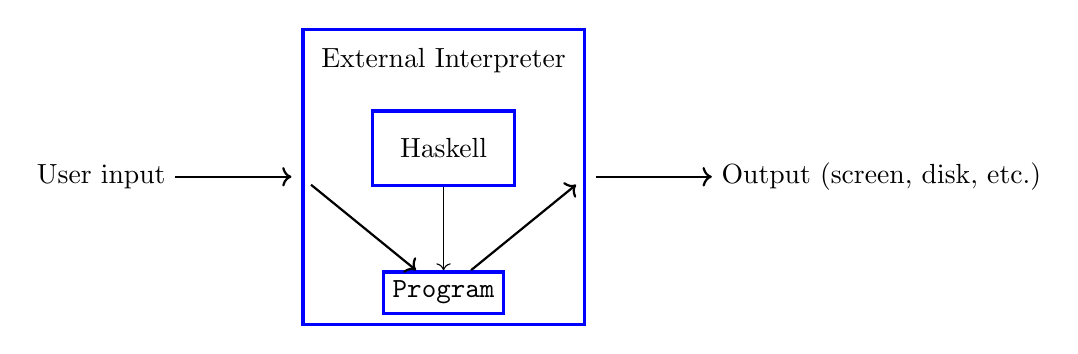
\begin{tikzpicture}[node distance = 1.6cm]
\node[matrix, draw=blue, very thick, row sep = 1em] (I)
{
\node{External Interpreter};\\
\node[draw, inner sep = 1em] (H) {Haskell};\\[2em]
\node[draw] (P) {\texttt{Program}};\\
};
\draw[->] (H)--(P);
\node (Inp) [left=of I] {User input};
\node (IL) at (I.west) {};
\draw[->, thick] (Inp) -- (IL);
\draw[->, thick] (IL) -- (P);
\node (Out) [right=of I] {Output (screen, disk, etc.)};
\node (IR) at (I.east) {};
\draw[->, thick] (P) -- (IR);
\draw[->, thick] (IR) -- (Out);
\end{tikzpicture}
\caption{Visual representation of the (fictitious) external interpreter connecting to Haskell to run a \lsin|Program|}\label{fig:program}
\end{figure}

One thing that we ought to be able to do with \lsin|Program|s is compose them. For example, suppose that we have a program \lsin|askName :: Program| and another \lsin|greet :: String -> Program|, the first of which asks the user for their name, and the second of which, given a name, will print `Hello, \textit{name}' on the screen. It is reasonable to want to build a composite program, \lsin|askAndGreet :: Program|, which asks the user for their name and proceeds to greet them. How could we define \lsin|askAndGreet| starting from \lsin|askName| and \lsin|greet|?

Unfortunately, we can't, because the \lsin|Program| abstraction is missing one critical thing: \lsin|Program|s are unable to pass the results of their computations onwards to other \lsin|Program|s. In this case, \lsin|askName| should be able to give its output (the user input) to \lsin|greet|. Therefore, we now allow a different kind of \lsin|Program|, which besides its implicit input and output (via effects on the world) also has an explicit output, which can be passed onwards to other \lsin|Program|s. This new kind of program is called \lsin|IO|, or rather, \lsin|IO a|, with \lsin|a| a Haskell type. To recap:
\begin{itemize}
\item A value of type \lsin|Program| is an instruction or sequence of instructions built by Haskell, which the external interpreter executes,
\item However, since this formalism does not have a built-in way to pass outcomes of some programs to others, we add a new type of program: \lsin|IO|.
\item A value of type \lsin|IO a|, with \lsin|a| a Haskell type, is an instruction or sequence of instructions built by Haskell, which the external interpreter executes, which culminates in a value of type \lsin|a|.
\end{itemize}

There is but one short hop before we understand how Haskell deals with side effects: the type \lsin|Program| does not actually exist. Indeed, a program which does not culminate in any value can be identified with a program that culminates in an object of a trivial type, such as \lsin|()|. For example, the Haskell function \lsin|putStrLn| is of type \lsin|String -> IO ()|.

\subsection{Working with \texorpdfstring{\texttt{IO}}{IO} and a few Examples}

Let us look at a couple of the simplest \lsin|IO| functions in Haskell:
\begin{lstlisting}
getLine :: IO String
putStrLn :: String -> IO ()
\end{lstlisting}

These types should be interpreted as: \lsin|getLine| is a program which goes off into the world and comes back to Haskell with a \lsin|String|, usually input that the user has written into the console. On the other hand, \lsin|putStrLn| isn't a program in its own right: it is a function which receives a \lsin|String| and returns a program, which in turn does some action on the outside world (printing the \lsin|String|) and returns no information.

\paragraph{Hello World}
Our first program with side effects will be the classical `Hello world!':
\begin{lstlisting}
main :: IO ()
main = putStrLn "Hello world!"
\end{lstlisting}

When compiled, this program results in an executable which, when run, prints the string `Hello world!' to the screen. Note the use of \lsin|main|. A Haskell file will typically define many functions, so we need to tell the compiler which of them builds the \lsin|IO ()| value it is meant to execute, so it looks for a value of type \lsin|IO ()| and name \lsin|main|.

\paragraph{Echo and Bind}
Let us now make a program which receives input from the user and repeats it back to them. To get the input from the user we want the \mbox{\lsin|IO String|} action \lsin|getLine|, and we want to feed its output (a \lsin|String|) to the \lsin|putStrLn| function. Unfortunately, it's not as easy as writing \lsin|putStrLn . getLine|, as \lsin|getLine| returns an \lsin|IO String| and \lsin|putStrLn| requires a \lsin|String|.

A `program composition operator' must behave as follows: given an \lsin|IO| action which culminates in a value of type \lsin|a|, and a function which turns such a value into another computation of type \lsin|IO b|, we want to write the program `do this thing, feed the \lsin|a| into this function, and do that other thing'. The operator that does this composition is called \emph{bind}:
\begin{lstlisting}
(>>=) :: IO a -> (a -> IO b) -> IO b
\end{lstlisting}

This is the tool necessary to do the echo program:
\begin{lstlisting}
main = getLine >>= putStrLn
\end{lstlisting}

\paragraph{Prompting and Prettying: Using Lambdas}

We will now make a less rude program. Instead of simply getting input and saying it right back like a petulant child, we will kindly ask the user for their name, and upon getting it with the use of \lsin|getLine|, we will return a greeting `Hello, \textit{name}!'.

First, we define the \lsin|IO ()| action which consists of prompting the user:
\begin{lstlisting}
askName :: IO ()
askName = putStrLn "Hello! What is your name?"
\end{lstlisting}

Then, we define a function which gets the user input and returns a greeting. To this effect, we need to modify the input (turning the name into a pretty message) before printing it. To do this, we could first define an auxilliary function, which is then composed with \lsin|getLine|:
\begin{lstlisting}
greet :: String -> IO ()
greet name = putStrLn ("Hello, " ++ name ++ "!")

getNameAndGreet :: IO ()
getNameAndGreet = getLine >>= greet
\end{lstlisting}

However, in order to avoid cluttering our code with functions that are only ever used once, it is sometimes better to instead use a lambda expression in place of \lsin|greet|:
\begin{lstlisting}
getNameAndGreet :: IO ()
getNameAndGreet = getLine >>= (\name -> putStrLn ("Hello, " ++ name ++ "!"))
\end{lstlisting}

Finally, we compose \lsin|askName| and \lsin|getNameAndGreet|. However, we cannot use \lsin|>>=|: for that to work, we would need that \lsin|getNameAndGreet| be of type \lsin|() -> IO ()|, and not \lsin|IO ()|. The fix is simple, however: instead of writing \lsin|getNameAndGreet| on the right-hand side of \lsin|>>=| we write a function which takes one argument of type \lsin|()|, ignores it, and returns the \lsin|IO| action \lsin|getNameAndGreet|.
\begin{lstlisting}
main = askName >>= (\x -> getNameAndGreet)
\end{lstlisting}

Of course, writing this is slightly silly and verbose for something as simple as `run this program then run this one', so Haskell offers an alternative, via the \lsin|>>| operator, which can be read as `and then':
\begin{lstlisting}
(>>) :: IO a -> IO b -> IO b
a1 >> a2 = a1 >>= (\x -> a2)
\end{lstlisting}

We may write our greeting program without any auxilliary functions, to see it in all its glory:
\begin{lstlisting}
main = putStrLn "Hello! What is your name?" >>
       getLine >>=
       (\name -> putStrLn ("Hello, " ++ name ++ "!"))
\end{lstlisting}


\paragraph{\texttt{IO} is a Functor}

In the previous example, we got user input and forwarded it using \lsin|>>=| to another function, which processed it and returned another \lsin|IO| action. However, sometimes it is appropriate to associate the processing to the left-hand side of \lsin|>>=| rather than to the right-hand side.

As an example, consider the following scenario: we wish to make a program that receives an integer input by the user, doubles it, and prints it on the screen. Let us take for granted that there exists a function \lsin|strToInt :: String -> Int| which reads an integer off of a string,\footnote{In Haskell, there is the \lsin|read| function which does just that, but it is unsafe as it crashes the program if it is fed invalid input. There are other, safer alternatives, but it should suffice to say that they exist.} as well as a function \lsin|print :: Int -> IO ()| which prints an integer to the screen.\footnote{Actually, the function \lsin|print| has type \lsin|print :: Show a => a -> IO ()|. The \lsin|Show| typeclass consists of types which may be represented as a string; to represent a value as a string one uses the function \lsin|show :: Show a => a -> String|. With it, one defines \lsin|print = putStrLn . show|.} Then, our program could be written as
\begin{lstlisting}
main = getLine >>= (print . (\x -> 2*x) . strToInt)
\end{lstlisting}


However, suppose that we want to isolate the `get an integer from the user' action. In other words, we want to build a Haskell object of type \lsin|IO Int|, using \lsin|getLine :: IO String| and \lsin|strToInt :: String -> Int|. We cannot simply construct a composite \lsin|strToInt . getLine|, as the types don't match, but if we could build a function \lsin|IO String -> IO Int| out of \lsin|strToInt| our problem would be solved. Interpreting this in the program framework, this function would take an \lsin|IO String|, i.e. a sequence of instructions for the external interpreter telling it how to fetch a \lsin|String| from the outside world, and add to the very end of these instructions `when you're done getting that \lsin|String|, apply the function \lsin|strToInt| to it'. 

This function exists, and can be constructed via \lsin|fmap strToInt|. Yes, this is the same \lsin|fmap| as in \ref{sec:functors}: \lsin|IO| is a functor! In other words, if we define a map $F \colon \Hask \to \Hask$ given by
\begin{itemize}
\item If $a$ is a type, $F(a) = \typecons{IO} a$,
\item If $f \colon a \to b$, define $F(f) \colon F(a) \to F(b)$ as in the previous paragraph,
\end{itemize}
then $F$ is a functor. In other words, \lsin|fmap| satisfies the functor laws.\footnote{Strictly speaking, this is not necessarily true. There might be a small difference between \lsin|action :: IO a| and \lsin|fmap id action|: the former is a sequence of instructions, and the latter is the same sequence \emph{followed by} `and then, apply \lsin|id| to the result'. Of course, this is obviously of no consequence, except perhaps for an infinitesimal delay in execution, and it is very likely that the compiler would optimize away such a frivolous instruction anyway. Regardless of whether there exists a difference or not, there is no harm in accepting the fiction that \lsin|IO| is a functor, in much the same way that engineers do not need to correct for relativistic effects when building bridges.}

In conclusion, we are now able to define an \lsin|IO Int| action which reads an integer from the console, as
\begin{lstlisting}
getInt :: IO Int
getInt = fmap strToInt getLine
\end{lstlisting}

\paragraph{The Monad Laws}

From the discussion above, we are able to conclude a very important fact relating \lsin|>>=| and \lsin|fmap| which will be very important later on: doing an \lsin|IO|-free computation before or after \lsin|>>=| is irrelevant. In other words, if \lsin|act1 = IO a|, \lsin|f :: a -> b| and \lsin|act2 = a -> IO b| then
\begin{equation}
\lsmath{act >>= (act2 . f) = (fmap f act) >>= act2}
\end{equation}

This is the most important of the so-called \emph{monad laws}, which will be heavily discussed in section \ref{sec:monads}.

\subsection{Conclusion}

In this section, we discussed what a value of type \lsin|IO a| is (it is a sequence of instructions for the interpreter to go out into the world and get Haskell an object of type \lsin|a|), how to compose \lsin|IO| actions with functions that take their results and return other \lsin|IO| actions via the \lsin|>>=| operator, and how \lsin|IO| is a functor.

The \lsin|>>=| operator changes the \lsin|IO| metaphor slightly, because it allows for the outside world to talk to Haskell. For example, consider the program
\begin{lstlisting}
main = getLine >>= (\in -> if in == "jackpot" then putStrLn "You hit the jackpot!" else putStrLn "...")
\end{lstlisting}

Then, when the interpreter executes this program, first it gets user input, and then it consults Haskell `hey, I got this input, what do I do now?', and Haskell replies with another \lsin|IO| action. Consequently, figure \ref{fig:program} could be improved, leading to figure \ref{fig:program2}, which represents Haskell not as a box which is executed once to yield a \lsin|Program|, but rather as an engine the interpreter is in constant conversation with, executing actions, showing their results to Haskell, and consulting it about what to do next.
\begin{figure}
\centering
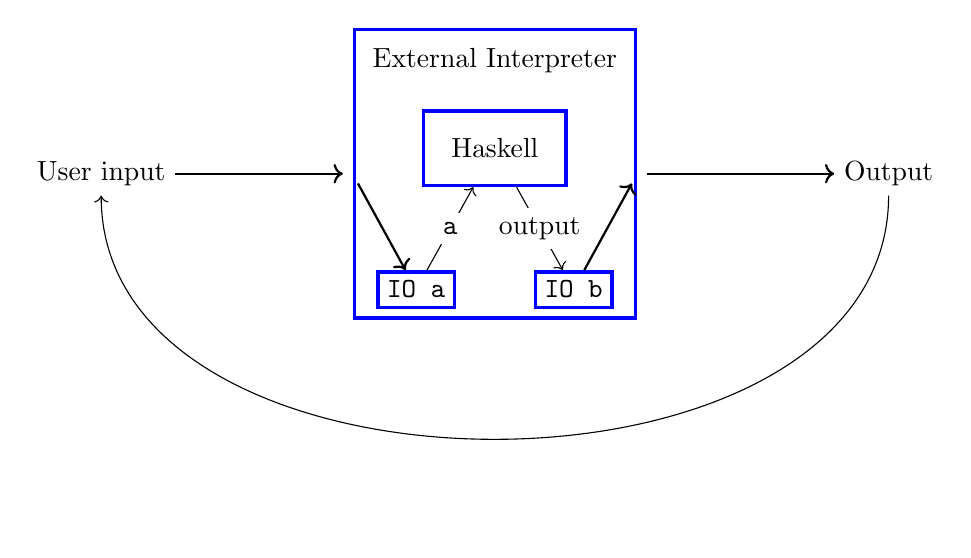
\begin{tikzpicture}[node distance = 1.6cm]
\node[matrix, draw=blue, very thick, row sep = 1em] (I) at (0,0)
{
\node{External Interpreter};\\
\node[draw, inner sep = 1em] (H) {Haskell};\\[2em]
\node[draw] (P1) at (-1,0) {\texttt{IO a}};
\node[draw] (P2) at (1,0) {\texttt{IO b}};\\
};
\draw[->] (P1)--(H) node[midway, fill=white] {\texttt{a}};
\draw[->] (H)--(P2) node[midway, fill=white] {output};
\node (Inp) at (-5,0) {User input};
\node (IL) at (I.west) {};
\draw[->, thick] (Inp) -- (IL);
\draw[->, thick] (IL) -- (P1);
\node (Out) at (5,0) {Output};
\node (IR) at (I.east) {};
\draw[->, thick] (P2) -- (IR);
\draw[->, thick] (IR) -- (Out);

\node (BO) [below=4cm of Out] {};
\node (BI) [below=4cm of Inp] {};

\draw[->] (Out) .. controls (BO) and (BI) .. (Inp);
\end{tikzpicture}
\caption{Visual representation of the ongoing conversation between Haskell and the (fictitious) interpreter}\label{fig:program2}
\end{figure}


\section{Monads}\label{sec:monads}

We preface this section with a joke.

\begin{joke}
\leavevmode
\begin{description}[labelindent=\parindent]
\item[Novice learning Haskell:] What is a Monad?

\item[Haskell expert:] Nothing special: it's just a monoid in the category of endofunctors!
\end{description}
\end{joke}

\subsection{Categorical Definition}

Before talking about the applications to programming, we give a very brief introduction to the concept of monad. For a more in depth but still light introduction, see chapter VI of \cite{maclane}.

\begin{definition}\label{def:monad}
A monad in a category $X$ is an endofunctor $T \colon X \to X$, together with two natural transformations
\begin{equation}
\eta \colon \id_X \nto T, \quad \mu \colon T^2 \nto T,
\end{equation}
satisfying the equations
\begin{gather}
\mu \cdot T\mu = \mu \cdot \mu T,\\
\mu \cdot \eta T = \mu \cdot T \eta = \id_T.
\end{gather}
\end{definition}

Monads often, but not always, arise from adjunctions.

\begin{prop}\label{prop:monadj}
Let $F \colon X \to Y$ and $U \colon Y \to X$ be adjoint functors, with $F \dashv U$. Then, $T = UF$ is a monad, with $\eta$ the unit of the adjunction and $\mu = U \varepsilon F$, where $\varepsilon$ is the counit of the adjunction.
\end{prop}

Let us look at one particular example, which will be useful in the sequence. Let $F \colon \cat{Sets} \to \cat{Mon}$ be the free-monoid-generated-by functor, and $U \colon \cat{Mon} \to \cat{Sets}$ the forgetful functor. In this case, $T = UF$ is the functor which, given a set $A$, returns the monad freely generated by $A$, without the monadic structure. In other words, we can see $T(A)$ as the collection of finite sequences of elements of $A$.

In this case, $\eta \colon A \to T(A)$ is the function which, given an element $a$ of $A$, returns the one-element sequence `$a$'.

The other natural transformation, $\mu$, is trickier. It is a function from $T(T(A))$ to $T(A)$. In other words, it receives sequences of sequences of elements of $A$, and returns a sequence of elements of $A$.\footnote{Strictly speaking, this is not necessarily true. The result is heavily dependent on how we represent the free monad generated by a set. Here we will be assuming that the free monad generated by $A$ is represented by the finite sequences of elements of $A$, with the operation given by concatenation.} It is not obvious, but can be deduced by expanding the definition of $\mu$ and $\eta$, that $\mu$ consists of sequence concatenation. In other words, suppose that $s = s_1 \dots s_n$ is an element of $T(T(A))$, with
\begin{equation}
s_i = a_{i1} \dots a_{i m_i}, \quad i = 1, \dots, n, \quad a_{ij} \in A.
\end{equation}

Then, $\mu(s)$ is given by
\begin{equation}
\mu(s) = a_{11} \dots a_{1 m_1} a_{21} \dots a_{2 m_2} \dots a_{n1} \dots a_{n m_n}.
\end{equation}

\subsection{A Monad in Haskell: Lists}

\paragraph{Lists as Sequences}

We have seen that a simple example of a monad consists of the functor which takes a set $A$ and returns the collection of finite sequences of elements of $A$. As it happens, we have already seen such an object in Haskell: the list functor!\footnote{This is not technically true. Since Haskell is lazy, it is possible (and oftentimes useful) to construct infinite lists. Therefore, the list functor does not correspond exactly to the monad associated to the free monoid constructor. However, it is close enough that the exposition does not suffer for it.}

The list functor $\type{List} \colon \Hask \to \Hask$ takes a type \lsin|a| and returns the type \lsin|[a]|, and it takes a function \lsin|f :: a -> b| and returns the function \lsin|fmap f :: [a] -> [b]| which applies \lsin|f| to all the elements of its input. To see it as a monad, by analogy with the example seen above we set
\begin{lstlisting}
eta :: a -> [a]
eta x = [x]

mu :: [[a]] -> [a]
mu = concat
\end{lstlisting}
where \lsin|concat| takes a list of lists and returns the result of their concatenation. This shows that Haskell already contains the natural transformation $\mu$ for the list functor, and it also contains $\eta$ in the form of the function \lsin|return :: a -> [a]|.

\paragraph{Lists as Output of Nondeterministic Computations}

An important example of list usage is when some query has more than one possible response. For some applications, only one response is enough, but sometimes it is useful to know all possible responses to a query.

As an example, consider the following game. Start with a composite integer $n$. At each step, pick a divisor $1 < d < n$ of $n$ and replace $n$ with $d-1$. The game halts whenever we reach a prime number $n$, or $1$. We wish to find, for a positive integer $n$, the maximal number of moves until the game halts.

To a first approximation, let us implement a simple strategy to play the game: at each step of the game we pick the biggest divisor of $n$. Our code will execute this strategy and return the number of moves necessary to halt.
\begin{lstlisting}
step :: Int -> Maybe Int
step n = let divisors = filter (\d -> n `mod` d == 0) [n-1,n-2..2] in
           fmap (\d -> d-1) (listToMaybe divisors)

stepsToHalt :: Int -> Int
stepsToHalt n = aux (step n)

aux :: Maybe Int -> Int
aux Nothing = 0
aux (Just n) = 1 + aux (step n)

stepsToHalt 73
output: 0

stepsToHalt 766
output: 8
\end{lstlisting}

Some explanation on the functions and notation used in the code above:
\begin{itemize}
\item The function \lsin|filter :: (a -> Bool) -> [a] -> [a]| takes a predicate \lsin|p| and a list \lsin|x| and returns the elements of the list which satisfy \lsin|p|. In this case the predicate is that \lsin|n `mod` d == 0|, i.e. that \lsin|d| be a divisor of \lsin|n|.

\item The expression \lsin|[n-1,n-2..2]| represents the list that is suggested by the notation.

\item The function \lsin|listToMaybe| takes a list and returns \lsin|Just| the first element of the list if it exists, and \lsin|Nothing| otherwise.
\end{itemize}

Now, evidently our strategy is not optimal. For example, suppose we start with $n = 48$. The current implementation goes $48 \to 23$, and so halts in one step. However, there is a better set of moves: $48 \to 15 \to 4 \to 1$.

With this in mind, let us implement a nondeterministic solver, where instead of picking a move and sticking with it, all possible moves are tried in parallel.

In preparation for this nondeterministic solver, we consider how to represent a state of the game at hand. There are two cases: either the game is still ongoing, in which case we want to store how many steps have elapsed since the start, and the value of $n$ we currently have; or the game has already terminated, in which case we just want to store how many steps it took us to get where we are.
\begin{lstlisting}
type UnhaltedState = (Int, Int)
type HaltedState = Int
type GameState = Either HaltedState UnhaltedState
\end{lstlisting}

Now, our nondeterministic step function takes an unhalted game and returns a list which contains all possible states of the game after one step; in the special case where the value of $n$ which is input is prime or 1, it returns a singleton list, representing that the only possible next step is to halt.
\begin{lstlisting}
stepND :: UnhaltedState -> [GameState]
stepND (s,n) = let divisors = filter (\d -> n `mod` d == 0) [n-1,n-2..2] in
               if divisors == [] then [Left s]
               else fmap (\d -> (Right (s+1,d-1))) divisors
\end{lstlisting}

Now we implement the function \lsin|stepsFromStateND|, which, given a state \lsin|s|, outputs all possible numbers of moves until halting:
\begin{lstlisting}
stepsFromStateND :: GameState -> [Int]
stepsFromStateND (Left s) = return s
stepsFromStateND (Right st) = concat (fmap stepsFromStateND (stepND st))
\end{lstlisting}

Finally, we may extract the maximum number of moves by using the \lsin|maximum| function.
\begin{lstlisting}
stepsToHaltND :: Int -> Int
stepsToHaltND n = maximum (stepsFromStateND (Right (0,n)))
\end{lstlisting}

We can see that the nondeterministic version does fare better than the deterministic version.
\begin{lstlisting}
filter (\(x,y,z) -> y<z)
 (fmap (\n -> (n, stepsToHalt n, stepsToHaltND n)) [1..100])
 
output: [(28,1,2),(36,1,2),(40,1,2),(48,1,3),(58,2,3),(60,1,3),(64,1,3),(74,2,3),(75,2,3),(76,1,3),(82,2,3),(84,1,3),(87,2,3),(88,1,3),(96,1,3),(98,2,4)]
\end{lstlisting}

\paragraph{Nondeterministic Functions as Kleisli Arrows}

In the previous example, we used monadic structure explicitly in the function \lsin|stepsFromStateND|. Now we present another way to look at the problem.

Recall that in section \ref{sec:kleisli} we introduced the idea of different function compositions. In that section, we considered functions of type \lsin|a -> Writer m b|, which took an input and returned an output together with a log, and defined the fish operator \lsin|<=<| which computes `logged functions' by composing their logs appropriately.

We will now do a similar thing: we will redefine the concept of function composition in order to allow for composition of nondeterministic functions.

To be more precise, suppose that \lsin|f :: a -> [b]| is a nondeterministic function, which takes an \lsin|a| as input and returns possibly many (or none) values of \lsin|b| as output. Likewise, let \lsin|g :: b -> [c]|. Then, we define the nondeterministic composition of \lsin|g| and \lsin|f| as
\begin{lstlisting}
(<=<) :: (b -> [c]) -> (a -> [b]) -> a -> [c]
g <=< f = \x -> concat (fmap g (f x))
\end{lstlisting}

Note the fact that we are reusing the fish operator. This is no accident: as it happens, \lsin|Writer m| is also a monad, and if we'll look at the typing of the fish operator in GHCi:
\begin{lstlisting}
:t (<=<)
output: (<=<) :: Monad m => (b -> m c) -> (a -> m b) -> a -> m c
\end{lstlisting}

In other words, the fish operator is defined for pairs of functions of types \lsin|b -> m c| and \lsin|a -> m b| with \lsin|m| a monad. We have already seen the implementation for lists, and we will see that it generalizes trivially for a general monad \lsin|m|.

We can rewrite the function \lsin|stepsFromStateND| using the fish operator:
\begin{lstlisting}
stepsFromStateND :: GameState -> [Int]
stepsFromStateND (Left s) = return s
stepsFromStateND (Right st) = (stepsFromStateND <=< stepND) st
\end{lstlisting}

\paragraph{Nondeterministic Input}

Let us look at a third way to see nondeterministic functions, which is often more useful for practical programming.

In practice, programmers don't always have the opportunity to write their functions as neat compositions of other functions. Sometimes dependencies are used multiple times, and it is much easier to store data in a variable and then reuse that variable multiple times than coming up with convoluted ways to carry the data across function compositions to where it needs to be. In other words, function application is useful.

This presents a problem to nondeterministic programming, because if \lsin|y :: [b]| is the (nondeterministic) output of a function \lsin|f :: a -> [b]|, and we want to feed \lsin|y| as input to another function \lsin|g :: b -> [c]|, simply writing \lsin|g y| will not do. We need some kind of new `nondeterministic function application' which, given nondeterministic input and a nondeterministic function, applies the function to all elements of the input.

Enter the bind operator, \lsin|>>=|. Yes, this is the same bind operator as in section \ref{sec:io}, but now it has type
\begin{lstlisting}
(>>=) :: [a] -> (a -> [b]) -> [b]
\end{lstlisting}
or, more generally,
\begin{lstlisting}
(>>=) :: Monad m => m a -> (a -> m b) -> m b
\end{lstlisting}

For lists, it is defined by
\begin{lstlisting}
(>>=) :: [a] -> (a -> [b]) -> [b]
y >>= g = concat (fmap g y)
\end{lstlisting}
and \lsin|stepsFromStateND| may be rewritten using bind:
\begin{lstlisting}
stepsFromStateND :: GameState -> [Int]
stepsFromStateND (Left s) = return s
stepsFromStateND (Right st) = stepND st >>= stepsFromStateND
\end{lstlisting}

\subsection{It All Ties Together (Categorically)}

We have seen that the $\type{List}$ type constructor is a monad, and from that we were able to define the fish operator \lsin|<=<| and the bind operator \lsin|>>=|. Now, we will show that the converse holds, so that, for example, \lsin|<=<| can be used to compose functions \lsin|a -> IO b| with \lsin|b -> IO c|, or that \lsin|>>=| can be used to feed a \lsin|Writer m a| into a function of type \lsin|Writer m b|. It is an interesting exercise to understand how these operations are interpreted, but for the sake of conciseness we will only show that the bind and fish operators induce different, but equivalent, ways to define monads.

\begin{theorem}\label{thm:mon1}
Let $X$ be a category. The following data are equivalent.
\begin{itemize}
\item A functor $T \colon X \to X$ together with natural transformations
\begin{equation}
\eta \colon I \Rightarrow T, \quad \mu \colon T^2 \Rightarrow T
\end{equation}
such that
\begin{gather}
\mu \cdot \mu T = \mu \cdot T \mu, \label{eq:mu1}\\
\quad \mu \cdot \eta T = \mu \cdot T \eta = \id_T. \label{eq:mu2}
\end{gather}

\item A functor $T \colon X \to X$, together with a natural transformation
\begin{equation}
\eta \colon I \Rightarrow T
\end{equation}
and an associative binary operation $(g,f) \mapsto g \odot f$, defined for $f, g \in X_1$ satisfying
\begin{equation}
f \colon x \to T y, \quad g \colon y \to T z,
\end{equation}
with $g \odot f \colon x \to Tz$, and such that for all such $f$ and $g$ we have
\begin{equation}
f \odot \eta_x = \eta_y \odot f = f.
\end{equation}

Furthermore, it relates to usual composition by
\begin{gather}
(h \odot g) \circ f = h \odot (g \circ f),\label{eq:odot3}\\
Th' \circ (g' \odot f') = Th' \odot (Tg' \circ f').\label{eq:odot4}
\end{gather}
whenever $f$, $g$ and $h$ compose appropriately, and likewise for $f'$, $g'$ and $h'$.

\item A functor $T \colon X \to X$, together with a natural transformation
\begin{equation}
\eta \colon I \Rightarrow T
\end{equation}
and an operator $\beta_{xy} \colon X(x, Ty) \to X(Tx, Ty)$ which satisfies
\begin{gather}
Tf = \beta_{xy}(\eta_y \circ f),\label{eq:beta1}\\
\beta_{xy}(f) \circ \eta_x = f,\label{eq:beta2}\\
\beta_{yz}(g) \circ \beta_{xy}(f) = \beta_{xz}(\beta_{yz}(g) \circ f).\label{eq:beta3}
\end{gather}
\end{itemize}
\end{theorem}

\begin{remark}
Before going through with the proof, it is worth it to look at how these concepts are reflected in Haskell.

All three of the definitions start with a functor and a natural transformation $\eta$. In Haskell, the functor is a type constructor, e.g. \lsin|[]|, \lsin|Writer m|, \lsin|IO|, and the $\eta$ is represented by the function \lsin|return :: a -> m a|.

The first definition contains an additional natural transformation, denoted $\mu$. In Haskell, this is represented by the function \lsin|join :: m m a -> m a|.

The second definition contains the binary operator $\odot$. In Haskell, this is represented by the fish operator \lsin|<=<|.

The third definition is the one which is a little further away from its Haskell counterpart. In Haskell, $\beta$ is represented by the bind operator
\begin{lstlisting}
(>>=) :: m a -> (a -> m b) -> m b
\end{lstlisting}
whose typing is not the same as $\beta$. To get from one to the other, one must first invert the order of the arguments, yielding the function
\begin{lstlisting}
(=<<) :: (a -> m b) -> (m a -> m b)
(=<<) = curry ((uncurry (>>=)) . swap)
\end{lstlisting}

This one maps directly to $\beta$.

The reason that this mental gymnastics is necessary is because the original typing of bind only makes sense in nice enough categories, namely those with exponentiation. The modified definition is more general, being applicable to any category.
\end{remark}

\begin{proof}
Since all definitions provide the functor $T$ and natural transformation $\eta \colon I \Rightarrow T$, it suffices to construct the following three pieces of data from one another: $\mu$, $\odot$, and $\beta$.

\begin{itemize}
\item (Build $\odot$ from $\mu$) Let $f \colon x \to T y$ and $g \colon y \to T z$. Then, set
\begin{equation}
g \odot f := \mu_z \circ Tg \circ f.
\end{equation}

We need to verify that $\odot$ is associative and that $\eta$ is a neutral element.

To show associativity, we compute $(h \odot g) \odot f$, for $f \colon x \to Ty$, $g \colon y \to Tz$ and $h \colon z \to Tw$:
\begin{equation}
\begin{aligned}
(h \odot g) \odot f &= \mu_w \circ T(h \odot g) \circ f\\
&= \mu_w \circ T\mu_w \circ TTh \circ Tg \circ f\\
&= \mu_w \circ \mu_{Tw} \circ TTh \circ Tg \circ f &&\text{(by \eqref{eq:mu1})}\\
&= \mu_w \circ Th \circ \mu_{z} \circ Tg \circ f &&\text{(Naturality)} \\
&= \mu_w \circ Th \circ (g \odot f)\\
&= h \odot (g \odot f).
\end{aligned}
\end{equation}

Now, we prove that $f \odot \eta_x = f$:
\begin{equation}
\begin{aligned}
f \odot \eta_x &= \mu_y \circ Tf \circ \eta_x\\
&= \mu_y \circ \eta_{Ty} \circ f &&\text{(Naturality)} \\
&= \id_{T y} \circ f &&\text{(by \eqref{eq:mu2})}\\
&= f.
\end{aligned}
\end{equation}

The proof that $\eta_y \odot f = f$ is similar, and so we turn to showing \eqref{eq:odot3}.
\begin{equation}
\begin{aligned}
(h \odot g) \circ f &= (\mu_w \circ Th \circ g) \circ f\\
&= \mu_z \circ Th \circ (g \circ f)\\
&= h \odot (g \circ f).
\end{aligned}
\end{equation}

Finally, we prove \eqref{eq:odot4}.
\begin{equation}
\begin{aligned}
Th \circ (g \odot f) &= Th \circ \mu_z \circ Tg \circ f \\
&= \mu_w \circ T^2 h \circ Tg \circ f && \text{(Naturality)}\\
&= Th \odot (Tg \circ f).
\end{aligned}
\end{equation}

The first part of the proof is complete. The rest of the proof is mostly similar algebraic manipulations, so we omit them when they are simple.

\item (Build $\beta$ from $\odot$) Simply set
\begin{equation}
\beta_{xy}(f) = f \odot \id_{Tx}.
\end{equation}

To prove \eqref{eq:beta1}, we compose with an appropriate identity:
\begin{equation}
\begin{aligned}
\beta(\eta_y \circ f) &= (\eta_y \circ f) \odot \id_{Tx} \\
&= T \id_y \circ (\eta_y \circ f) \odot \id_{Tx}\\
&= T \id_y \odot (T\eta_y \circ Tf \circ \id_{Tx})&&\text{(by \eqref{eq:odot4})}\\
&= T \id_y \odot (T\eta_y \circ Tf)\\
&= T \id_y \circ (\eta_y \odot Tf)&&\text{(by \eqref{eq:odot4})}\\
&= f.
\end{aligned}
\end{equation}

The proof of \eqref{eq:beta2} is trivial, so we now prove \eqref{eq:beta3}:
\begin{equation}
\begin{aligned}
\beta(g) \circ \beta(f) &= (g \odot \id_{Ty}) \circ (f \odot \id_{Tx})\\
&= g \odot (f \odot \id_{Tx}) && \text{(by \eqref{eq:odot3})}\\
&= (g \odot f) \odot \id_{Tx}) && \text{(Associativity)}\\
&= ((g \odot \id_{Ty}) \circ f) \odot \id_{Tx} && \text{(by \eqref{eq:odot3})}\\
&= \beta(\beta(g) \circ f).
\end{aligned}
\end{equation}

\item (Build $\mu$ from $\beta$) Define $\mu_x$, for $x \in X_0$, by
\begin{equation}
\mu_x = \beta(\id_{Tx}).
\end{equation}

The proofs of naturality of $\mu$ and \eqref{eq:mu1} and \eqref{eq:mu2} are left to the reader.
\end{itemize}

Now that we have constructed $\odot$ from $\mu$, $\beta$ from $\odot$ and $\mu$ from $\beta$, it remains to show that these constructions preserve information. In other words, if we start from $\mu$, build $\odot$, then $\beta$, and then a new $\overline{\mu}$, we need to show that $\mu = \overline{\mu}$, and likewise for the other two constructions. The proof of this fact is straight-forward and left to the reader.
\end{proof}

\begin{remark}
It should be noted that the proof of theorem \ref{thm:mon1} gives us more than the statement: it actually tells us how to construct each piece of data from the others. This translates to implementation. For example, in Haskell a monad is defined in terms of the bind operator \lsin|>>=| (in the nomenclature above, $\beta$), and the fish operator \lsin|<=<| (in the notation above, $\odot$) is defined on all monads using bind.
\end{remark}

\begin{remark}
The definition in terms of $T$, $\eta$ and $\beta$ can actually be further simplified. Indeed, by \eqref{eq:beta1} the definition of $T$ on morphisms can be induced solely from the rest of the data. Therefore, if we remove the hypothesis that $T$ is a functor and replace the hypothesis \eqref{eq:beta1} by something else, we actually obtain a leaner definition of monad:

\begin{theorem}\label{thm:mon2}
Let $X$ be a category. The following data is equivalent:
\begin{itemize}
\item A monad $(T, \eta, \beta)$,
\item A map $T \colon X_0 \to X_0$, a collection of maps $\eta_x \colon x \to Tx$, and a collection of maps $\eta_{xy} \colon X(x, Ty) \to X(Tx,Ty)$, satisfying the so-called \emph{monad laws}:
\begin{gather}
\beta(\eta) = \id,\label{eq:betaeta}\\
\beta(f) \circ \eta = f,\\
\beta(g) \circ \beta(f) = \beta(\beta(g) \circ f).
\end{gather}
\end{itemize}
\end{theorem}

\begin{proof}
Evidently a monad induces such data. On the other hand, from this data we may define $T$ on morphisms via \eqref{eq:beta1}, and functoriality of the resulting $T$ is easy to verify; note that \eqref{eq:betaeta} is necessary to prove that $T(\id) = \id$.
\end{proof}

Theorem \ref{thm:mon2} is actually the reason behind an interesting historical accident. As it happens, functors and monads were both introduced in version 1.3 of the Haskell report (the official standard for the language), in 1996. Now, it was already known all the way back to 1989\footnote{See \cite{moggi1}, definition 3.2.1 (which corresponds to our definition via $\beta$) and proposition 3.2.4 (which establishes the equivalence between this definition and the classical one based on on functors). See also \cite{kleisli} for another proof of equivalence, way back in 1964.} that every monad was a functor, but it was only in 2015, with the so-called `\lsin|Applicative => Monad| proposal' (AMP) \cite{amp}, that the language itself enforced that \lsin|fmap| be defined for every instance of \lsin|Monad|. 
\end{remark}

\subsection{How Programming Inspires Math}

When we introduced monads in definition \ref{def:monad} we remarked (proposition \ref{prop:monadj}) that every adjunction induces a monad. On the other hand, it has been known since at least 1964 \cite{kleisli} that every monad is induced by an adjunction.

Historically, this all happened long before monads were applied to programming languages, but as it happens the work we have done leaves us but a short step away from this theorem.

We begin by remarking that every monad induces a category in a natural way: if we combine theorem \ref{thm:mon1} with ideas from definition \ref{def:kleisli}, we conclude that, given a monad $M = (T,\eta,\odot)$ on $T$, the collections
\begin{equation}
W_0 = X_0, \quad W(x,y) = X(x,Ty)
\end{equation}
form a category $W$ with $\odot$ as the composition and $\eta$ as the identities. This is called the \emph{Kleisli category for the monad $M$}. We may define $F \colon X \to W$ and $U \colon W \to X$ as
\begin{equation}\label{eq:fudef}
\begin{aligned}
&F(x) = x, && F(f) = \eta_y \circ f,\\
&U(x) = Tx, && U(f) = \beta(f) = f \odot \id_{Tx}.
\end{aligned}
\end{equation}

It is worth it to take a step back and interpret $W$, $F$ and $U$ in computational terms, and the list monad $T$ is particularly enlightening in this respect. We saw that a function \lsin|a -> [b]| can be interpreted as a nondeterminstic functions, and hence in this case \emph{the Kleisli category is the category whose morphisms are nondeterministic functions}, with the appropriate composition. The functor $F$ takes a deterministic function and turns it into a `deterministic nondeterministic function', whose list of outputs contains only one element. On the other hand, the functor $U$ takes a nondeterministic function and turns it into a deterministic function, by seeing the nondeterministic results for what they are: lists. In breaking the nondeterministic metaphor, it must turn a function in $W(x,y)$ into a function whose output is a nondeterministic $y$, i.e. $U \colon W(x,y) \to X(?, Ty)$. By consistency, $U$ must act on all objects by $T$, and we have already seen that $\beta$ acts on $W(x,y) = X(x,Ty)$ in an appropriate way. Interpreting $\beta$ computationally, $U$ goes to a category which does not know how to perform nondeterministic computations, so $U$ itself teaches the functions how to accept nondeterministic inputs using $\beta$.

Anyway, it is not too difficult to verify that $F$ and $U$ form an adjoint pair, which in turn originates the monad we started with. We already have the candidate for the unit, which is $\eta$, and so all that remains is to find the candidate for the counit, i.e. to solve the equation
\begin{equation}\label{eq:mufeu}
\mu_x = U(\varepsilon_{F(x)}).
\end{equation}

Expanding \eqref{eq:mufeu} using \eqref{eq:fudef}, we obtain
\begin{equation}
\mu_x = \beta(\varepsilon_{x}),
\end{equation}
and so we may use equation \eqref{eq:beta2} to recover $\varepsilon$ via
\begin{equation}
\varepsilon_y = \beta(\varepsilon_y) \circ \eta_{Ty} = \mu_y \circ \eta_{Ty},
\end{equation}
and hence, by \eqref{eq:mu2},
\begin{equation}
\varepsilon_y = \id_{Ty}.
\end{equation}

It is not difficult to show that $\eta$ and $\varepsilon$ satisfy the triangular equalities, and therefore $(F, U, \eta, \varepsilon)$ forms an adjunction, whose associated monad is $M$. Therefore, we have just shown:

\begin{theorem}
Every monad is induced by an adjunction in the sense of proposition \ref{prop:monadj}.
\end{theorem}

The proof that we have presented is due to Kleisli \cite{kleisli}. It is not the only construction; see for example VI.2 in \cite{maclane} for another, due to Eilenberg-Moore.

\section{Closing Remarks}

The connection between Haskell and category theory is a rather interesting one, and not only for its content. First of all, it is of note that we have barely touched on the computational part of the theory behind Haskell, such as lambda calculus and type theory. Those are interesting areas in their own right, and they have a remarkable intersection with category theory, for example when it comes to theorems for free \cite{theoremsforfree}. Furthermore, in this essay we have been working with `idealized Haskell', in which all functions terminate and there are no infinite loops or errors, which is of course an unreasonable assumption; domain theory helps us account for this, by providing better descriptions of what kind of thing can be output by a program. For example, formally, each type is inhabited by at least one element, called bottom and denoted $\bot$. This type represents a computation which does not terminate, and since Haskell is a \emph{lazy} language (a term which we have not had the opportunity to define or explore) the notion of bottom is more nuanced than it would seem at first sight. For example, the pair $(\bot, \bot)$ is different from $(\bot, 1)$, which is different from $(\bot, 2)$, and all of these are different from $\bot$ (the undefined pair).

Another interesting thing about using mathematics to describe Haskell is that it approaches physics in a sense. This is because Haskell is a \emph{real} programming language, and the real world is messy. Haskell is riddled with minor exceptions, concessions to practicality which break otherwise ironclad rules: the reader will have noticed that this essay is riddled with footnotes saying `well, actually...' In this sense, any description of Haskell (short of the official documentation) will be only an approximation, and much like how Newtonian and relativistic physics both have their place as descriptions of the world to better or worse approximation, so do idealized Haskell and more complex models. In this way, the content of this essay is applied category theory in a quite literal sense, which goes to show that even the most abstract areas of mathematics may eventually find application in the real world.

As a last remark on category theory, in this essay we have gone to reasonable depth on monads in particular as a programming abstraction. No other categorical concept has found as wide application, except of course for the notion of morphism and perhaps the notion of functor, but that does not mean that other categorical concepts go unused. For a great reference, see \cite{catforprog}, in which concepts such as comonads and coalgebras are used as a formalism for, for example, random number generation and object inspection (lenses), both of which very useful notions in practice.

\bibliographystyle{plain}
\bibliography{bibliography}

\end{document}